\documentclass[tikz]{standalone}
%\usetikzlibrary{calc}
\begin{document}


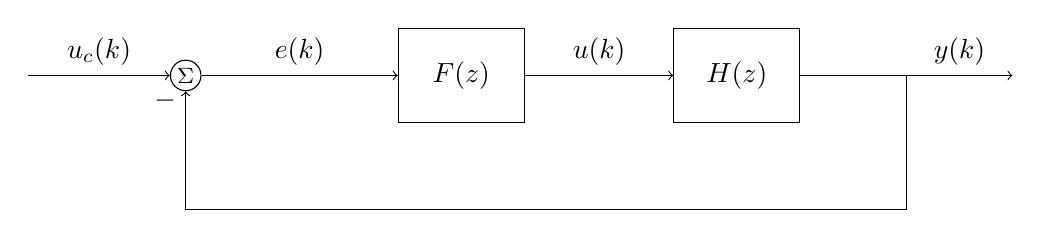
\begin{tikzpicture}[node distance=2cm, block/.style={rectangle, draw, minimum height=12mm, minimum width=16mm}, sumnode/.style={circle, draw, inner sep=1pt}]
  \node[coordinate] (input) {};
  \node[sumnode, right of=input] (sum) {\footnotesize $\Sigma$};
  \node[block,right of=sum, node distance=35mm] (control) {$F(z)$};
  \node[block,right of=control, node distance=35mm] (plant) {$H(z)$};
  \node[coordinate, right of=plant, node distance=35mm] (output) {};

  \draw[->] (input) -- node[above] {$u_c(k)$} (sum);
  \draw[->] (sum) -- node[above] {$e(k)$} (control);
  \draw[->] (control) -- node[above] {$u(k)$} (plant);
  \draw[->] (plant) -- node[coordinate] (feedback) {} node[near end, above] {$y(k)$} (output);
  \draw[->] (feedback) |- ++(0,-17mm) -| (sum) node[left, pos=0.96] {$-$};

\end{tikzpicture}
\end{document}
